\chapter{Porovnání účinnosti komprese dat ve formátu XML a JSON}
\label{kapitolaPorovnaniUcinnosti}
Poslední kapitola této diplomové práce je zaměřena na aplikaci vybraných kompresních mechanismů na data zapsaná ve formátech XML a JSON. Porovnání bylo provedeno na volně dostupných datech pomocí volně dostupných programů a algoritmů. Naměřené výsledky jsou popsány ve druhé části kapitoly.

\section{Technická parametry testování}

\subsection{Popis zvolených algoritmů}
Pro vzájemné porovnání jsem kromě algoritmů LZ77, XMill, JSONH a CJSON, které jsou popsány v částech \ref{lz77}, \ref{xmill}, \ref{jsonh} a \ref{cjson}, zvolil i algoritmy LZMA2, PPMd, gzip, které nejsou závislé na formátu dat. Program XMill byl spouštěn s požadovanými parametry z~příkazové řádky, algoritmus CJSON byl spouštěn v prohlížečí Google Chrome a mnou implementované algoritmy LZ77 a JSONH byly spouštěny jako konzolová aplikace referencující vytvořenou knihovnu. Zbývající 3 algoritmy implementuje program 7-Zip \cite{7zip}, který umožňuje volbu parametrů komprese, jako jsou velikosti slovníku, slova apod.

\begin{description}
\item[LZMA2] Jde o vylepšenou a optimalizovanou verzi LZ77, která využívá range kodéru a Markovových řetězců (viz \cite{introductionToDataCompression}). Stejně jako LZ77 využívá slovníku, pro který lze uživatelsky zvolit velikost slovníku i slova. Proti ostatním algoritmům alokuje při kompresi podstatně více paměti.
\item[PPMd] Tato statistická kompresní metoda pracuje s několika modely zároveň. Modely slouží k výpočtu pravděpodobnosti výskytu následujících znaků, které jsou kódovány aritmetickým kódováním (viz \cite{introductionToDataCompression}).
\item[gzip] Tento algoritmus je postaven na programu Deflate, který kombinuje LZ77 a Huffmanovo kódování. Nejprve jsou pomocí LZ77 odstraněny opakující se fráze a poté je výstup ještě zakódován Huffmanovým kódováním. 
\end{description}

\subsection{Popis testovacích souborů}
Testovací data bylo pro účely porovnání nutné získat zapsaná pomocí XML i JSON. Vybraná testovací data jsou volně dostupná ke stažení a to buď přímo ve formátu XML, nebo jako databáze. V prvním případě jsem data transformoval do formátu JSON pomocí frameworku Json.NET \cite{jsonNET}, ve druhém jsem soubory XML i JSON vytvořil. Velikost souborů je volena tak, aby bylo možné provést transformaci, a struktura dat je pro účely testování v každém souboru jedinečná. U popisu jednotlivých souborů uvádím hloubku zanoření, tzn. počet do sebe vnořených elementů pro XML nebo objektů a polí pro JSON.

\begin{description}
\item[base64img]Soubor 29 obrázků zakódovaných jako řetězec v soustavě o základu 64 popsaných pomocí tří údajů. Hloubka zanoření: 2.\\
Zdroj: Testovací soubory přiložené k XMill
\item[dblp]
Nehomogenní kolekce bibliografických údajů o periodikách z oblasti počítačových věd. Hloubka zanoření: až 6.\\
Zdroj: Testovací soubory přiložené k XMill
\item[Employees]
Data z databáze AdventureWorks2008R2 vybraná pomocí příkazu SELECT obsahují 7 převážně textových údajů o 19972 lidech. Hloubka zanoření: 2.\\
Zdroj: \texttt{msftdbprodsamples.codeplex.com/releases/view/93587}
\item[nasa]
Astronomická data agentury NASA, jde o převážně textová data s údaji o katalozích. Počet elementů 476646, počet atributů: 56317, hloubka zanoření XML: až 8.\\
Zdroj: \texttt{cs.washington.edu/research/xmldatasets/www/repository.html\#nasa}
\item[SigmodRecord]
Bibliografické údaje o článcích ze stránky sigmod.org. Jsou to převážně textová data -- název článku, jména autorů atd. Hloubka zanoření: 6.\\
Zdroj: \texttt{dia.uniroma3.it/Araneus/Sigmod/}
\end{description}

\section{Výsledky testování}
Testované algoritmy, které dovolují nastavit parametry, byly spuštěny několikrát pro různé kombinace parametrů. Z naměřených dat bylo vypozorováno, že při zvyšování hodnot parametrů existuje jistá mez, za kterou se velikost zkomprimovaného souboru snižuje již nevýznamně. Přitom však při kompresi platí mezi velikostí parametrů a množstvím spotřebované paměti přímá úměra, hodnoty parametrů je tedy vhodné volit s rozmyslem.

\subsection{Velikost komprimovaných souborů}
V grafech na obrázcích \ref{base64img}, \ref{dblp}, \ref{Employees}, \ref{nasa} a \ref{SigmodRecord} jsou uvedeny nejlepší dosažené výsledky komprimace pro jednotlivé soubory a algoritmy. Pro všechny soubory platí, že nejúčinněji je komprimovala metoda PPMd. Naopak pro 4 soubory obsahující JSON podávala nejhorší výsledky metoda CJSON. To je dáno stejně jako v případě metody JSONH tím, že komprimované soubory jsou validní JSON a obsahují pouze jiným způsobem zapsaná původní data. Na obhajobu těchto algoritmů musím uvést, že jejich primární použití je při zpracování dat JavaScriptem a zde hraje validita komprimovaných dat nespornou roli. Pomineme-li algoritmy specializované pro zpracování JSON a mnou implementované LZ77, dosahuje ve většině případů nejhorších anebo druhých nejhorších výsledků pro oba dva formáty dat metoda gzip kombinující LZ77 a Huffmanovo kódování. Metoda XMill, která využívá ke kompresi jednotlivých vytvořených bloků právě gzip, podávala proměnlivé výsledky: ve dvou případech byla mírně horší než gzip, ve třech naopak výrazně lepší. V~žádném případě však nedosáhla nejlepšího výsledku i pro různé volby kompresorů, což je poněkud překvapivé, ale může to být způsobeno nevhodným výběrem testovacích dat, která jsou převážně textová.

Zvláštním případem jsou soubory base64img (viz obrázek \ref{base64img}), u kterých nelze pozorovat typicky menší velikost dat v JSON. U těchto souborů bylo dosaženo nejmenšího kompresního poměru, který je zároveň pro všechny algoritmy mimo JSONH a CJSON přibližně konstantní. Tento jev je velice pravděpodobně způsoben obsahem souborů: obrázky zapsanými jako řetězce 64znakové abecedy. Například pro formát JSON zabírají tyto řetězce více než 95 \% obsahu souboru, čemuž odpovídá kompresní poměr (viz tabulka \ref{tabulkaKompresniPomer}) blízký hodnotě 1.

Na zbývajících čtyřech grafech (obrázky \ref{dblp}, \ref{Employees}, \ref{nasa} a \ref{SigmodRecord}) lze pozorovat proměnlivé výsledky jednotlivých algoritmů, což odpovídá rozdílné struktuře dat v souborech a tomu, že každý algoritmus využívá kombinaci jiných kompresních technik.

\begin{figure}[!h]
\centering
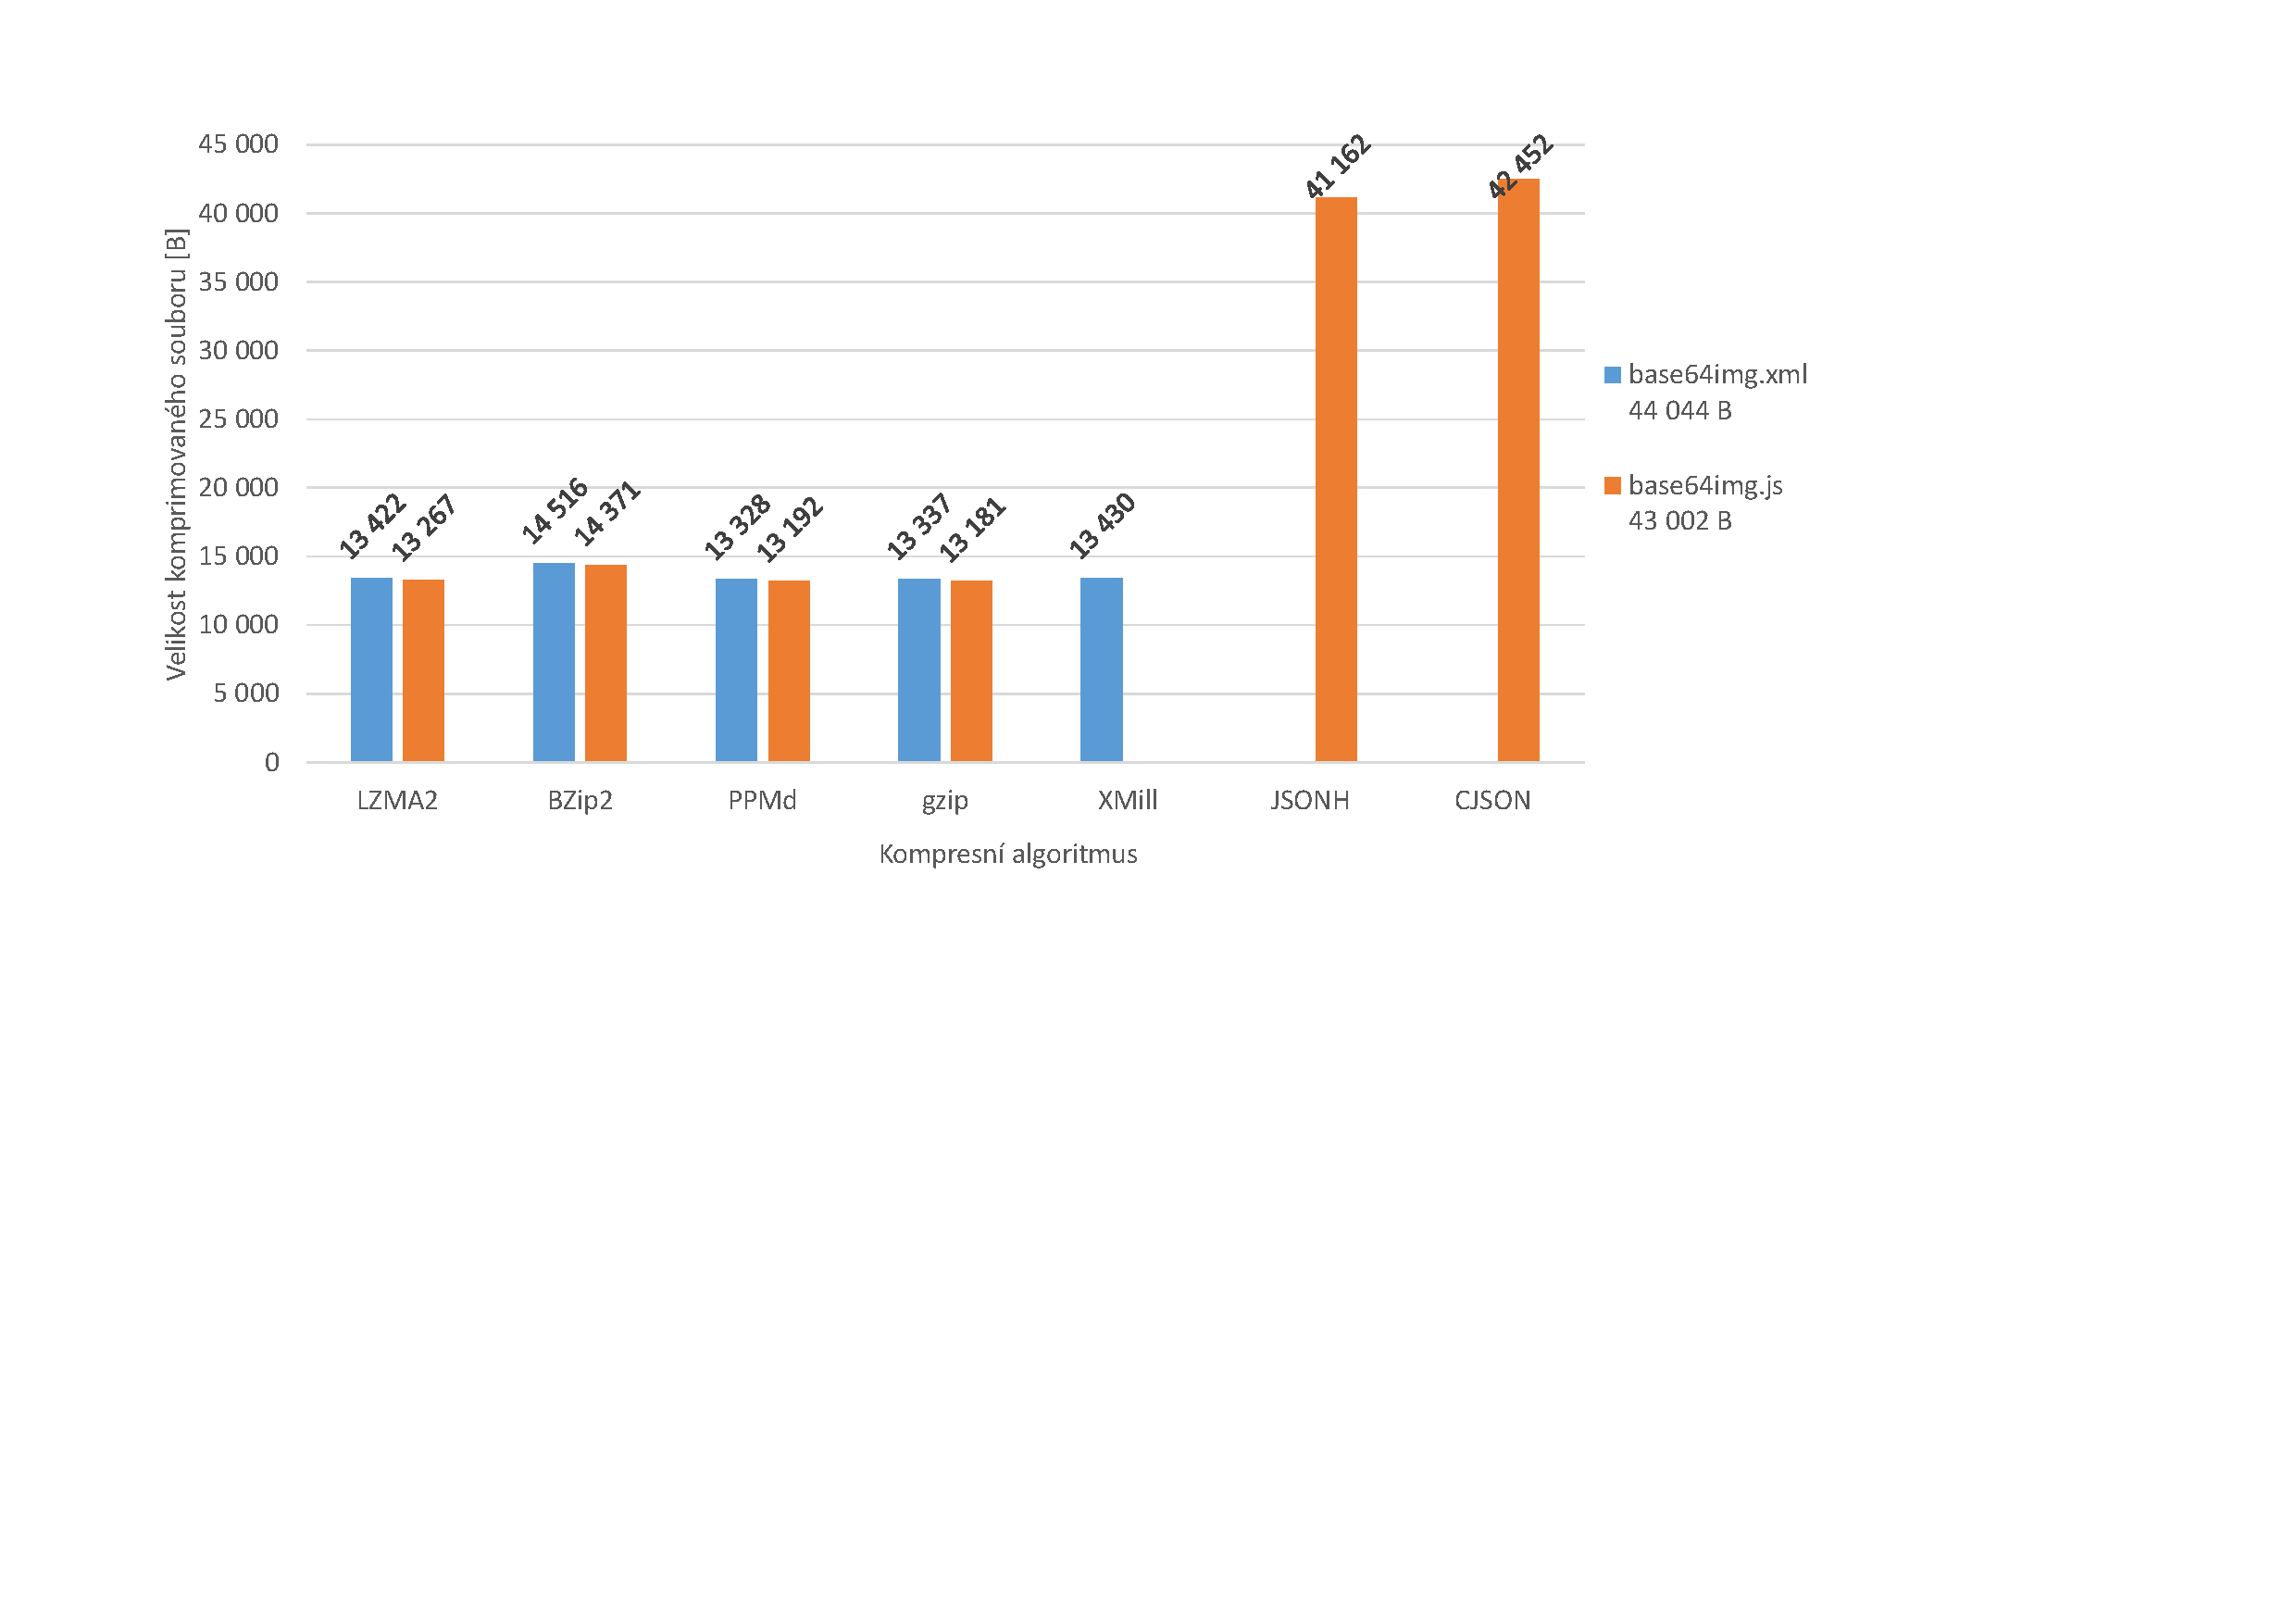
\includegraphics[trim=70 395 200 60, clip, angle=0, width=150mm]{base64img}
\caption{Velikost komprimovaných souborů base64img.xml a base64img.js}
\label{base64img}
\end{figure}

\begin{figure}[!h]
\centering
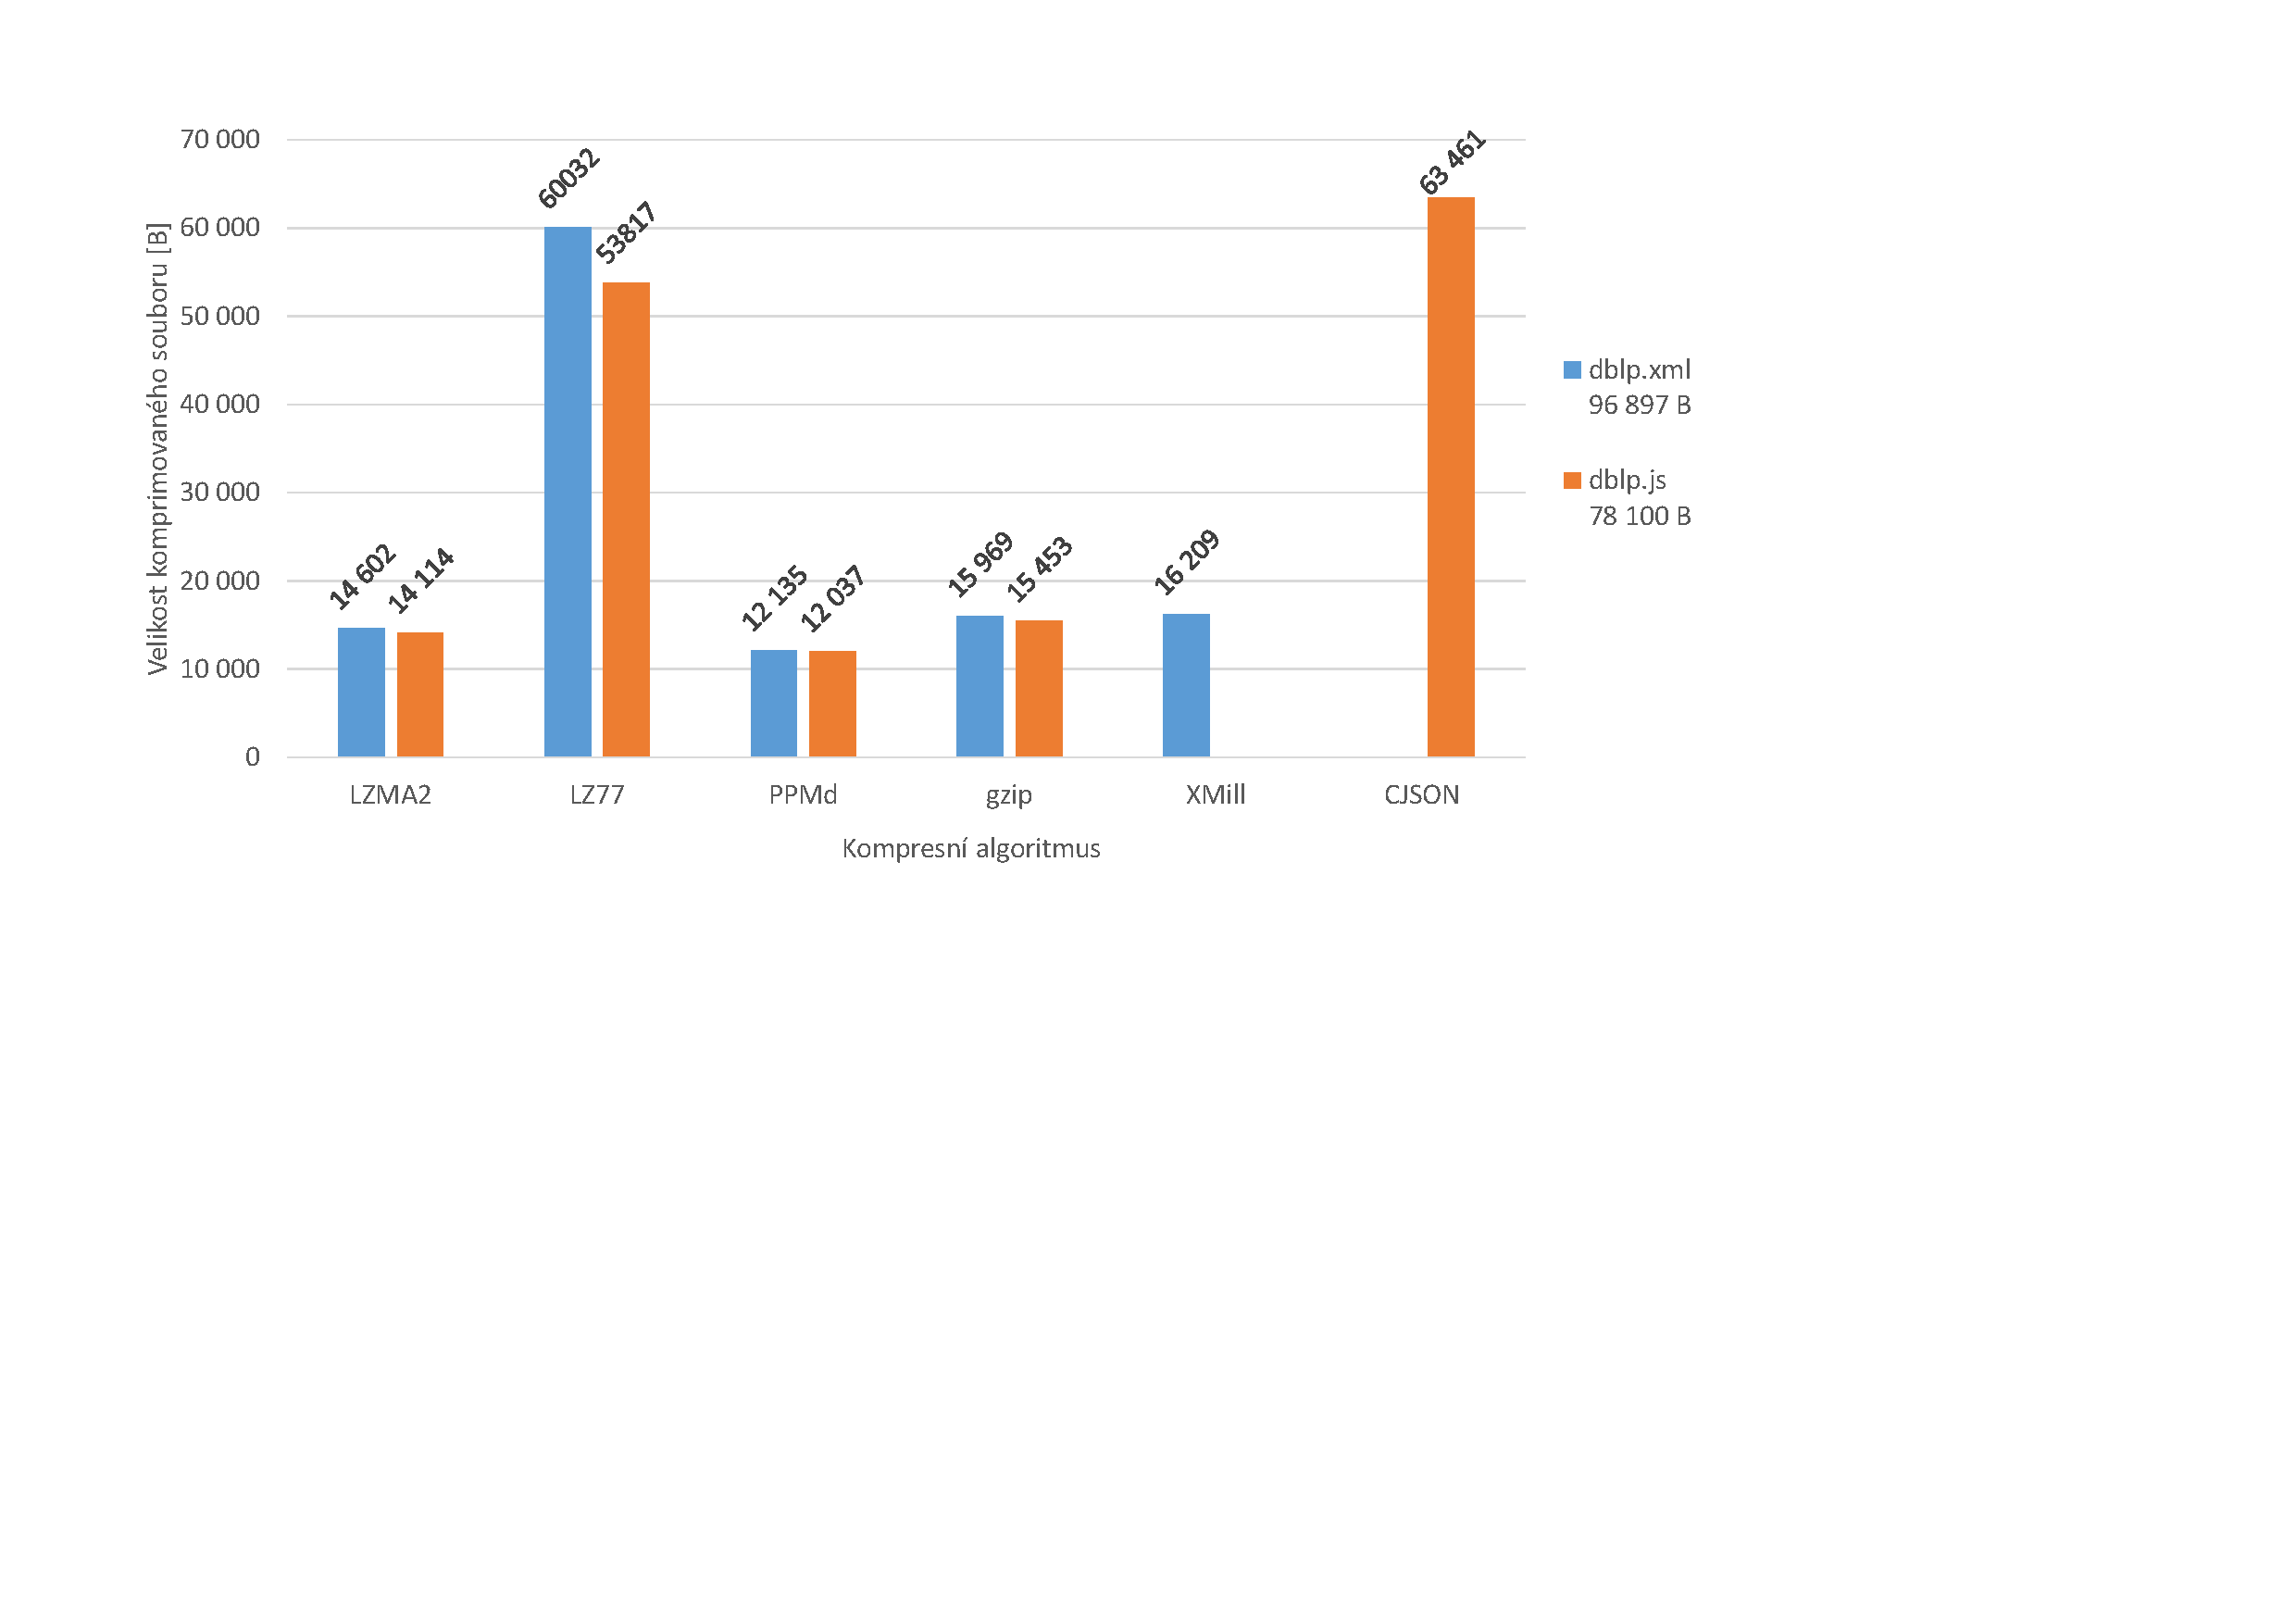
\includegraphics[trim=65 395 260 50, clip, angle=0, width=140mm]{dblp}
\caption{Velikost komprimovaných souborů dblp.xml a dblp.js}
\label{dblp}
\end{figure}

\begin{figure}[!h]
\centering
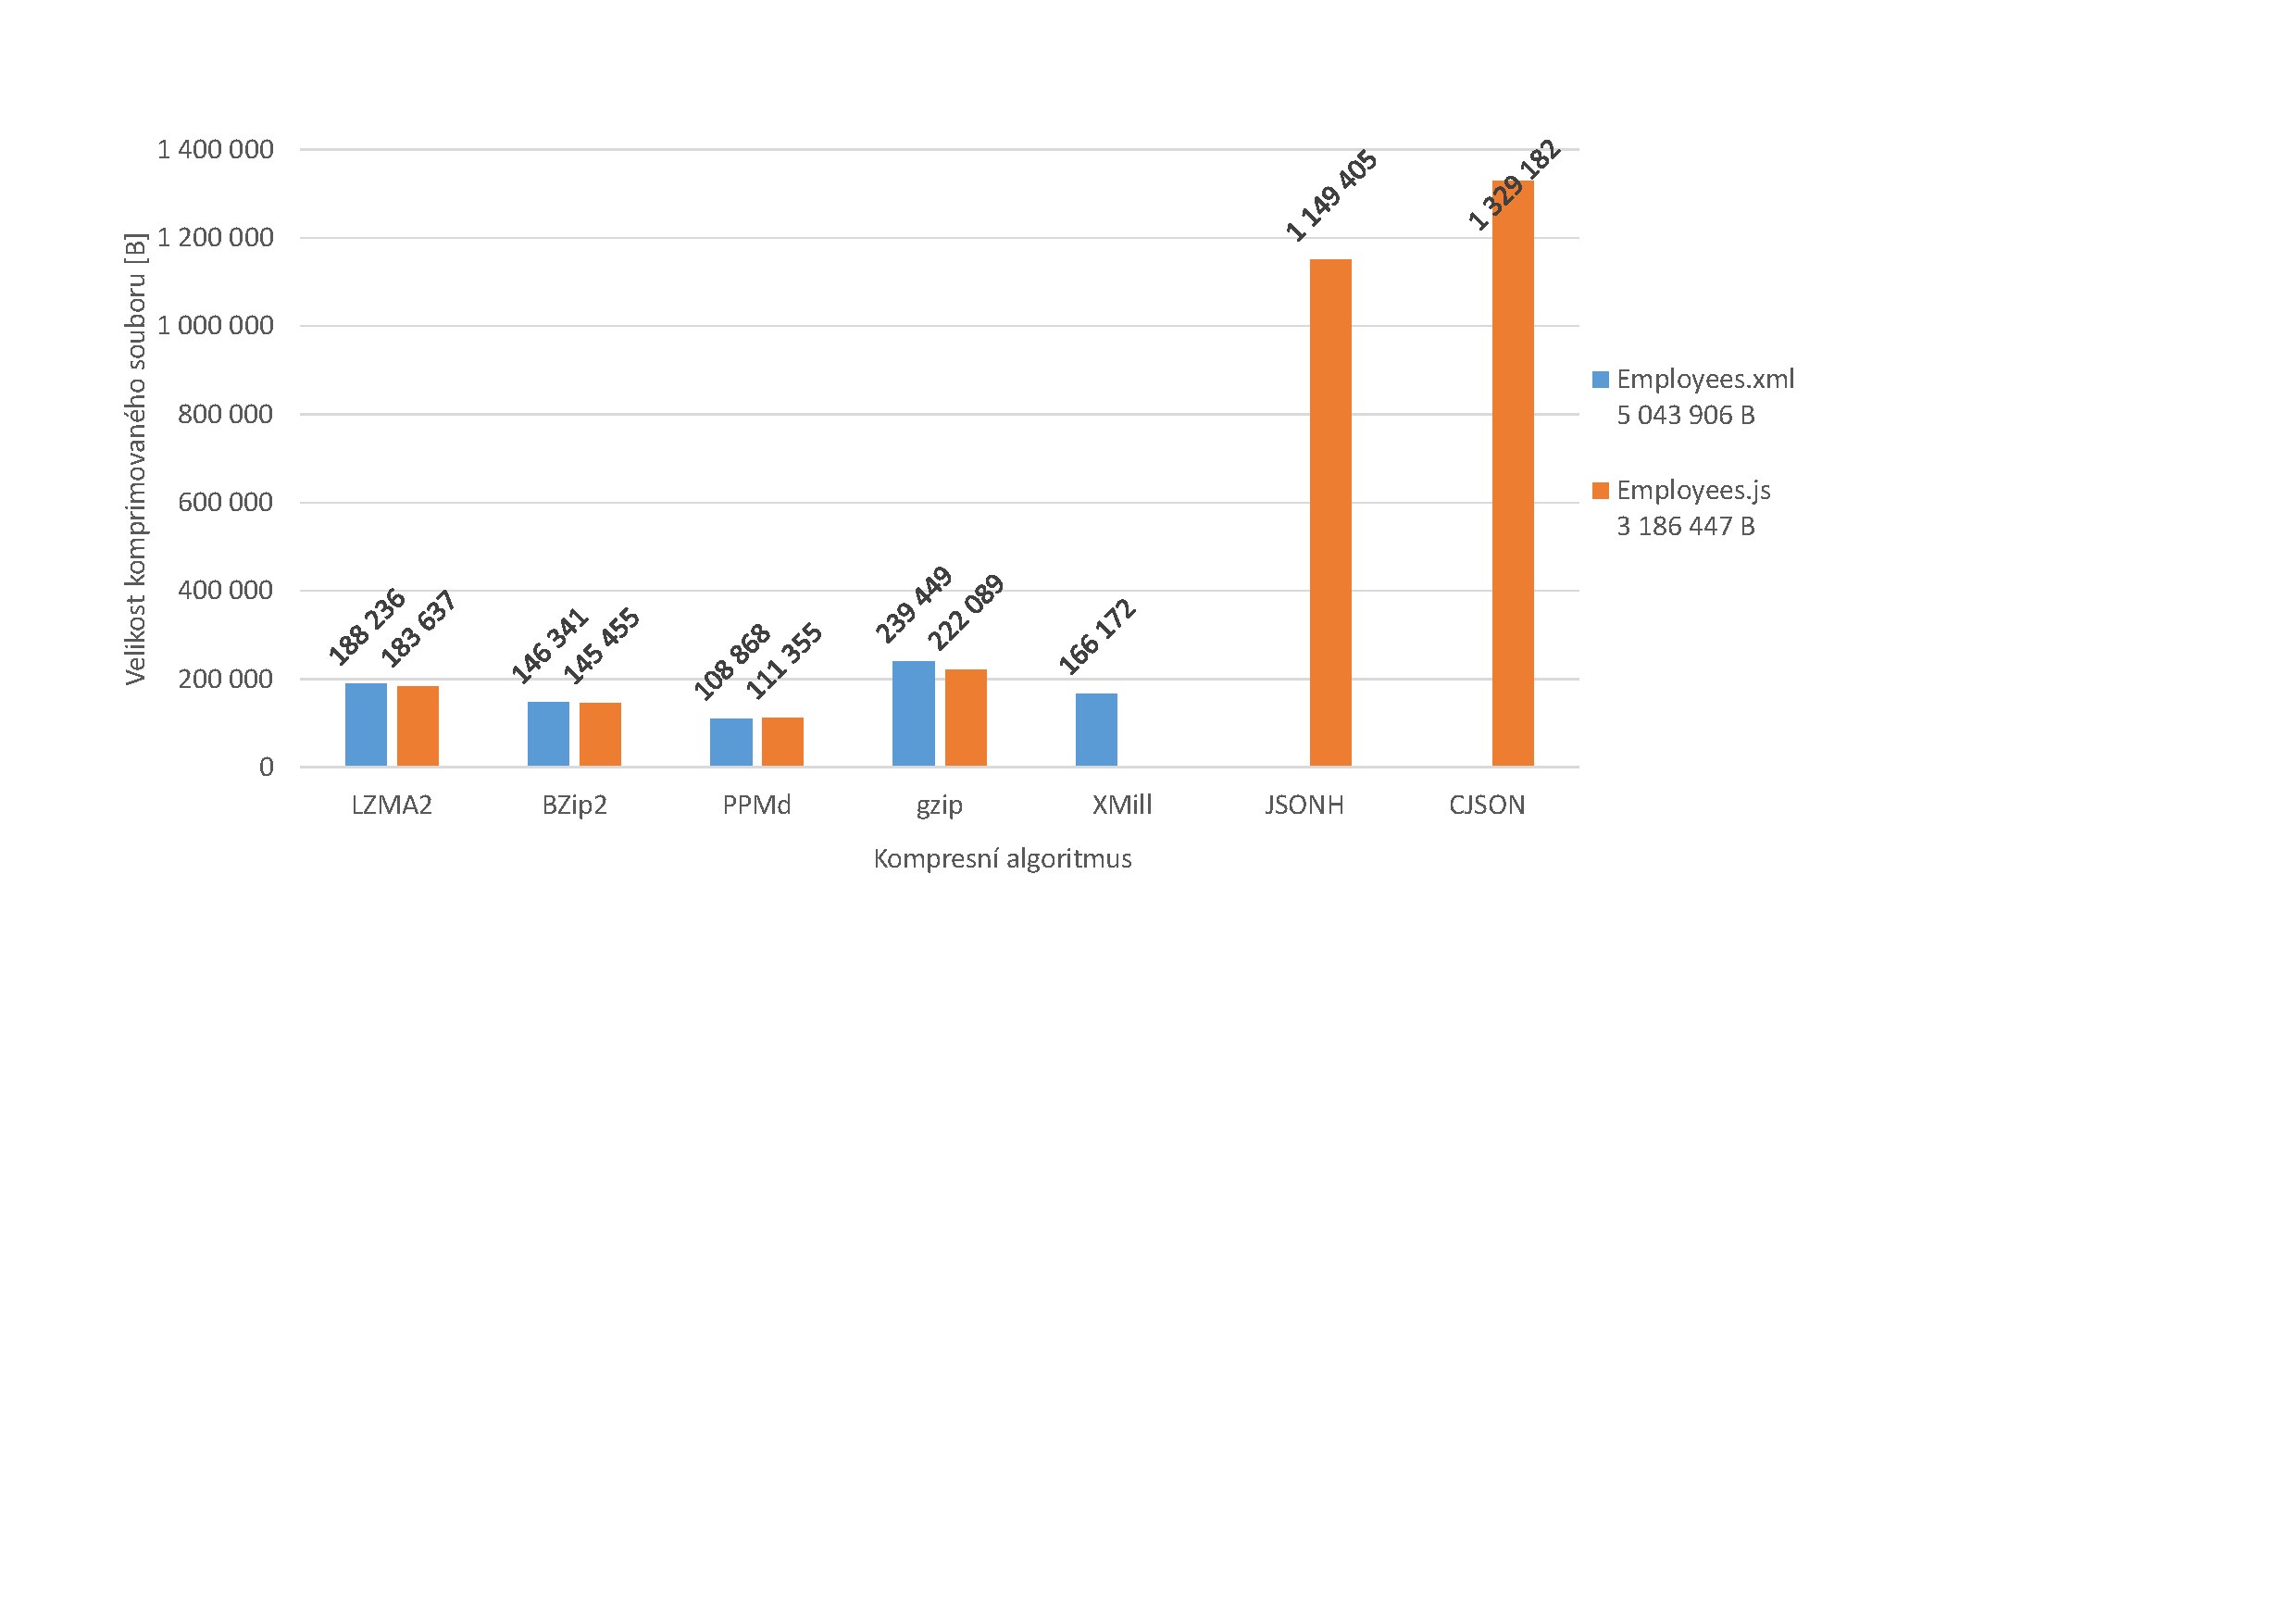
\includegraphics[trim=65 390 240 70, clip, angle=0, width=150mm]{Employees}
\caption{Velikost komprimovaných souborů Employees.xml a Employees.js}
\label{Employees}
\end{figure}

\begin{figure}[!h]
\centering
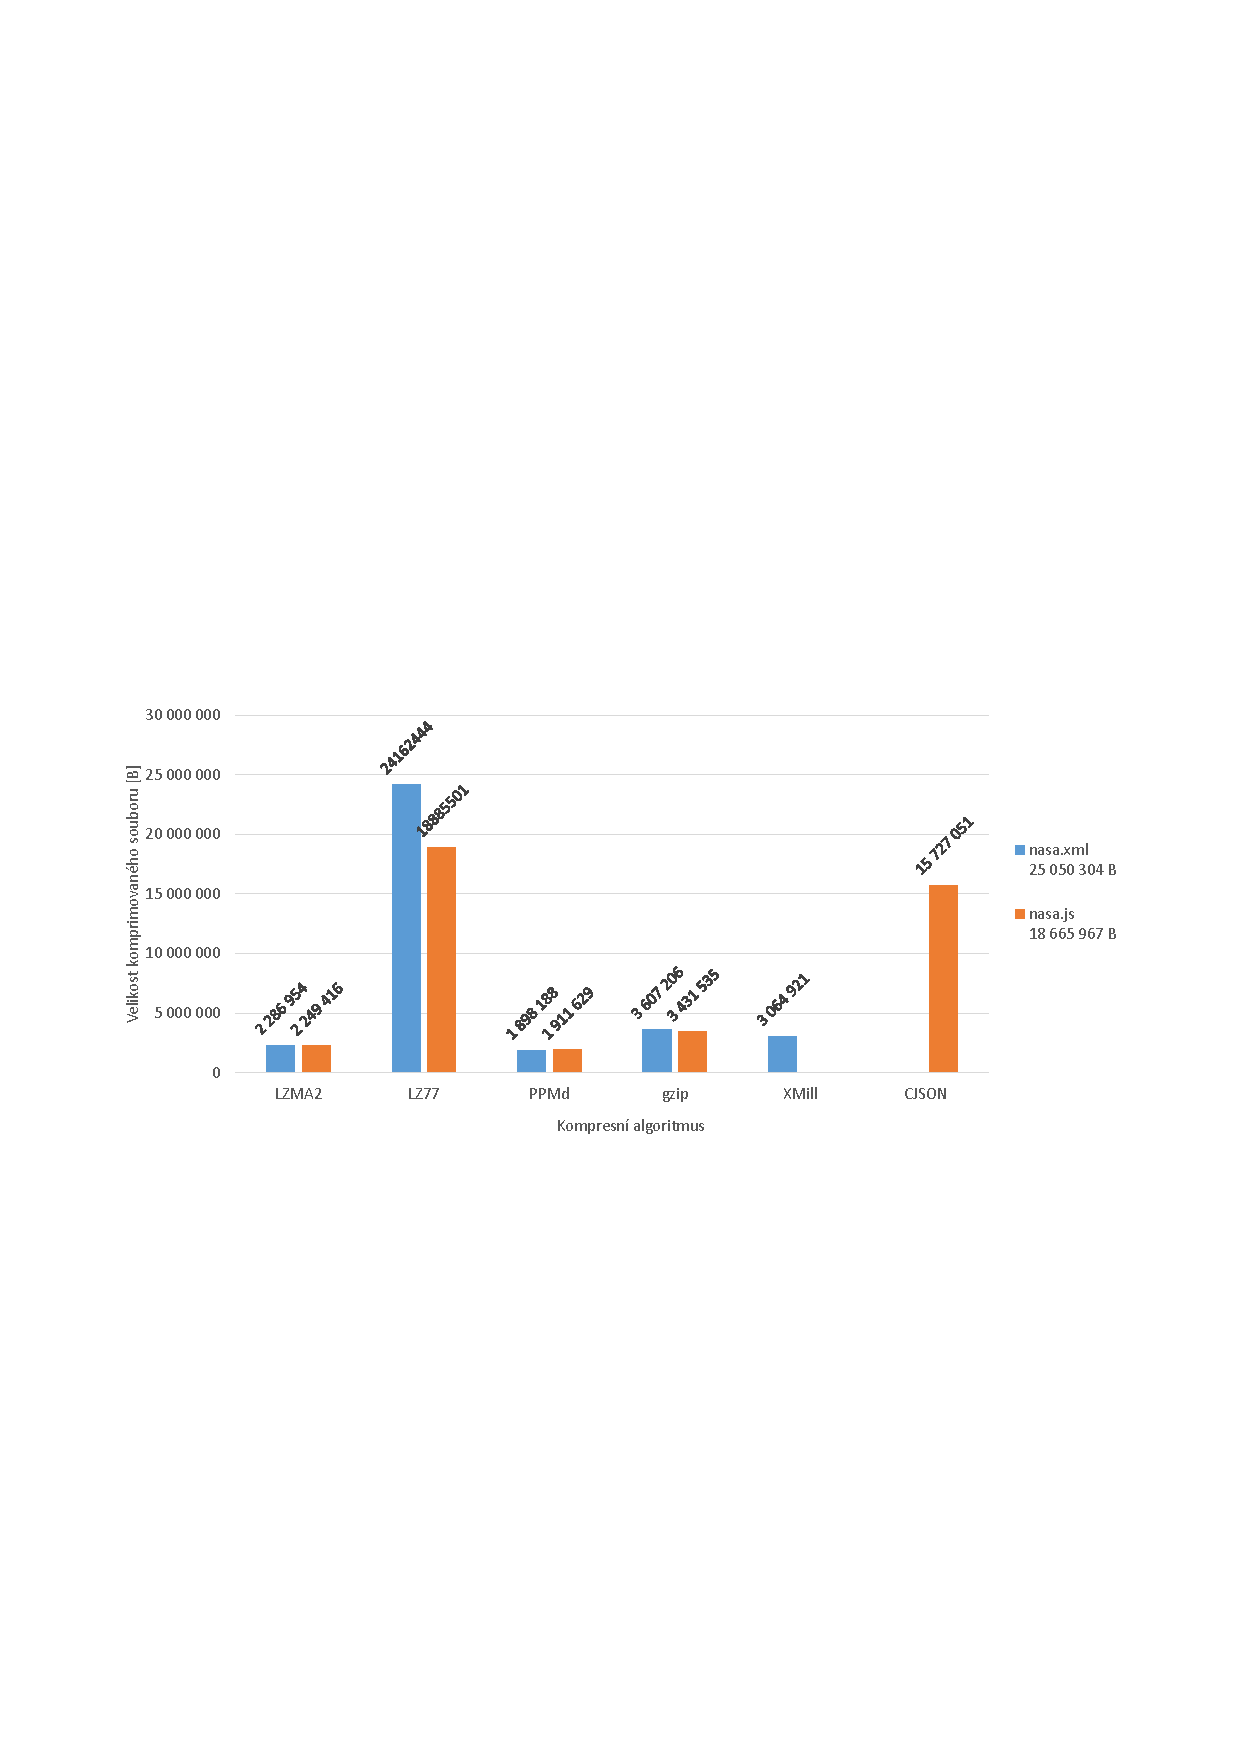
\includegraphics[trim=50 295 70 330, clip, angle=0, width=140mm]{nasa}
\caption{Velikost komprimovaných souborů nasa.xml a nasa.js}
\label{nasa}
\end{figure}

\begin{figure}[!h]
\centering
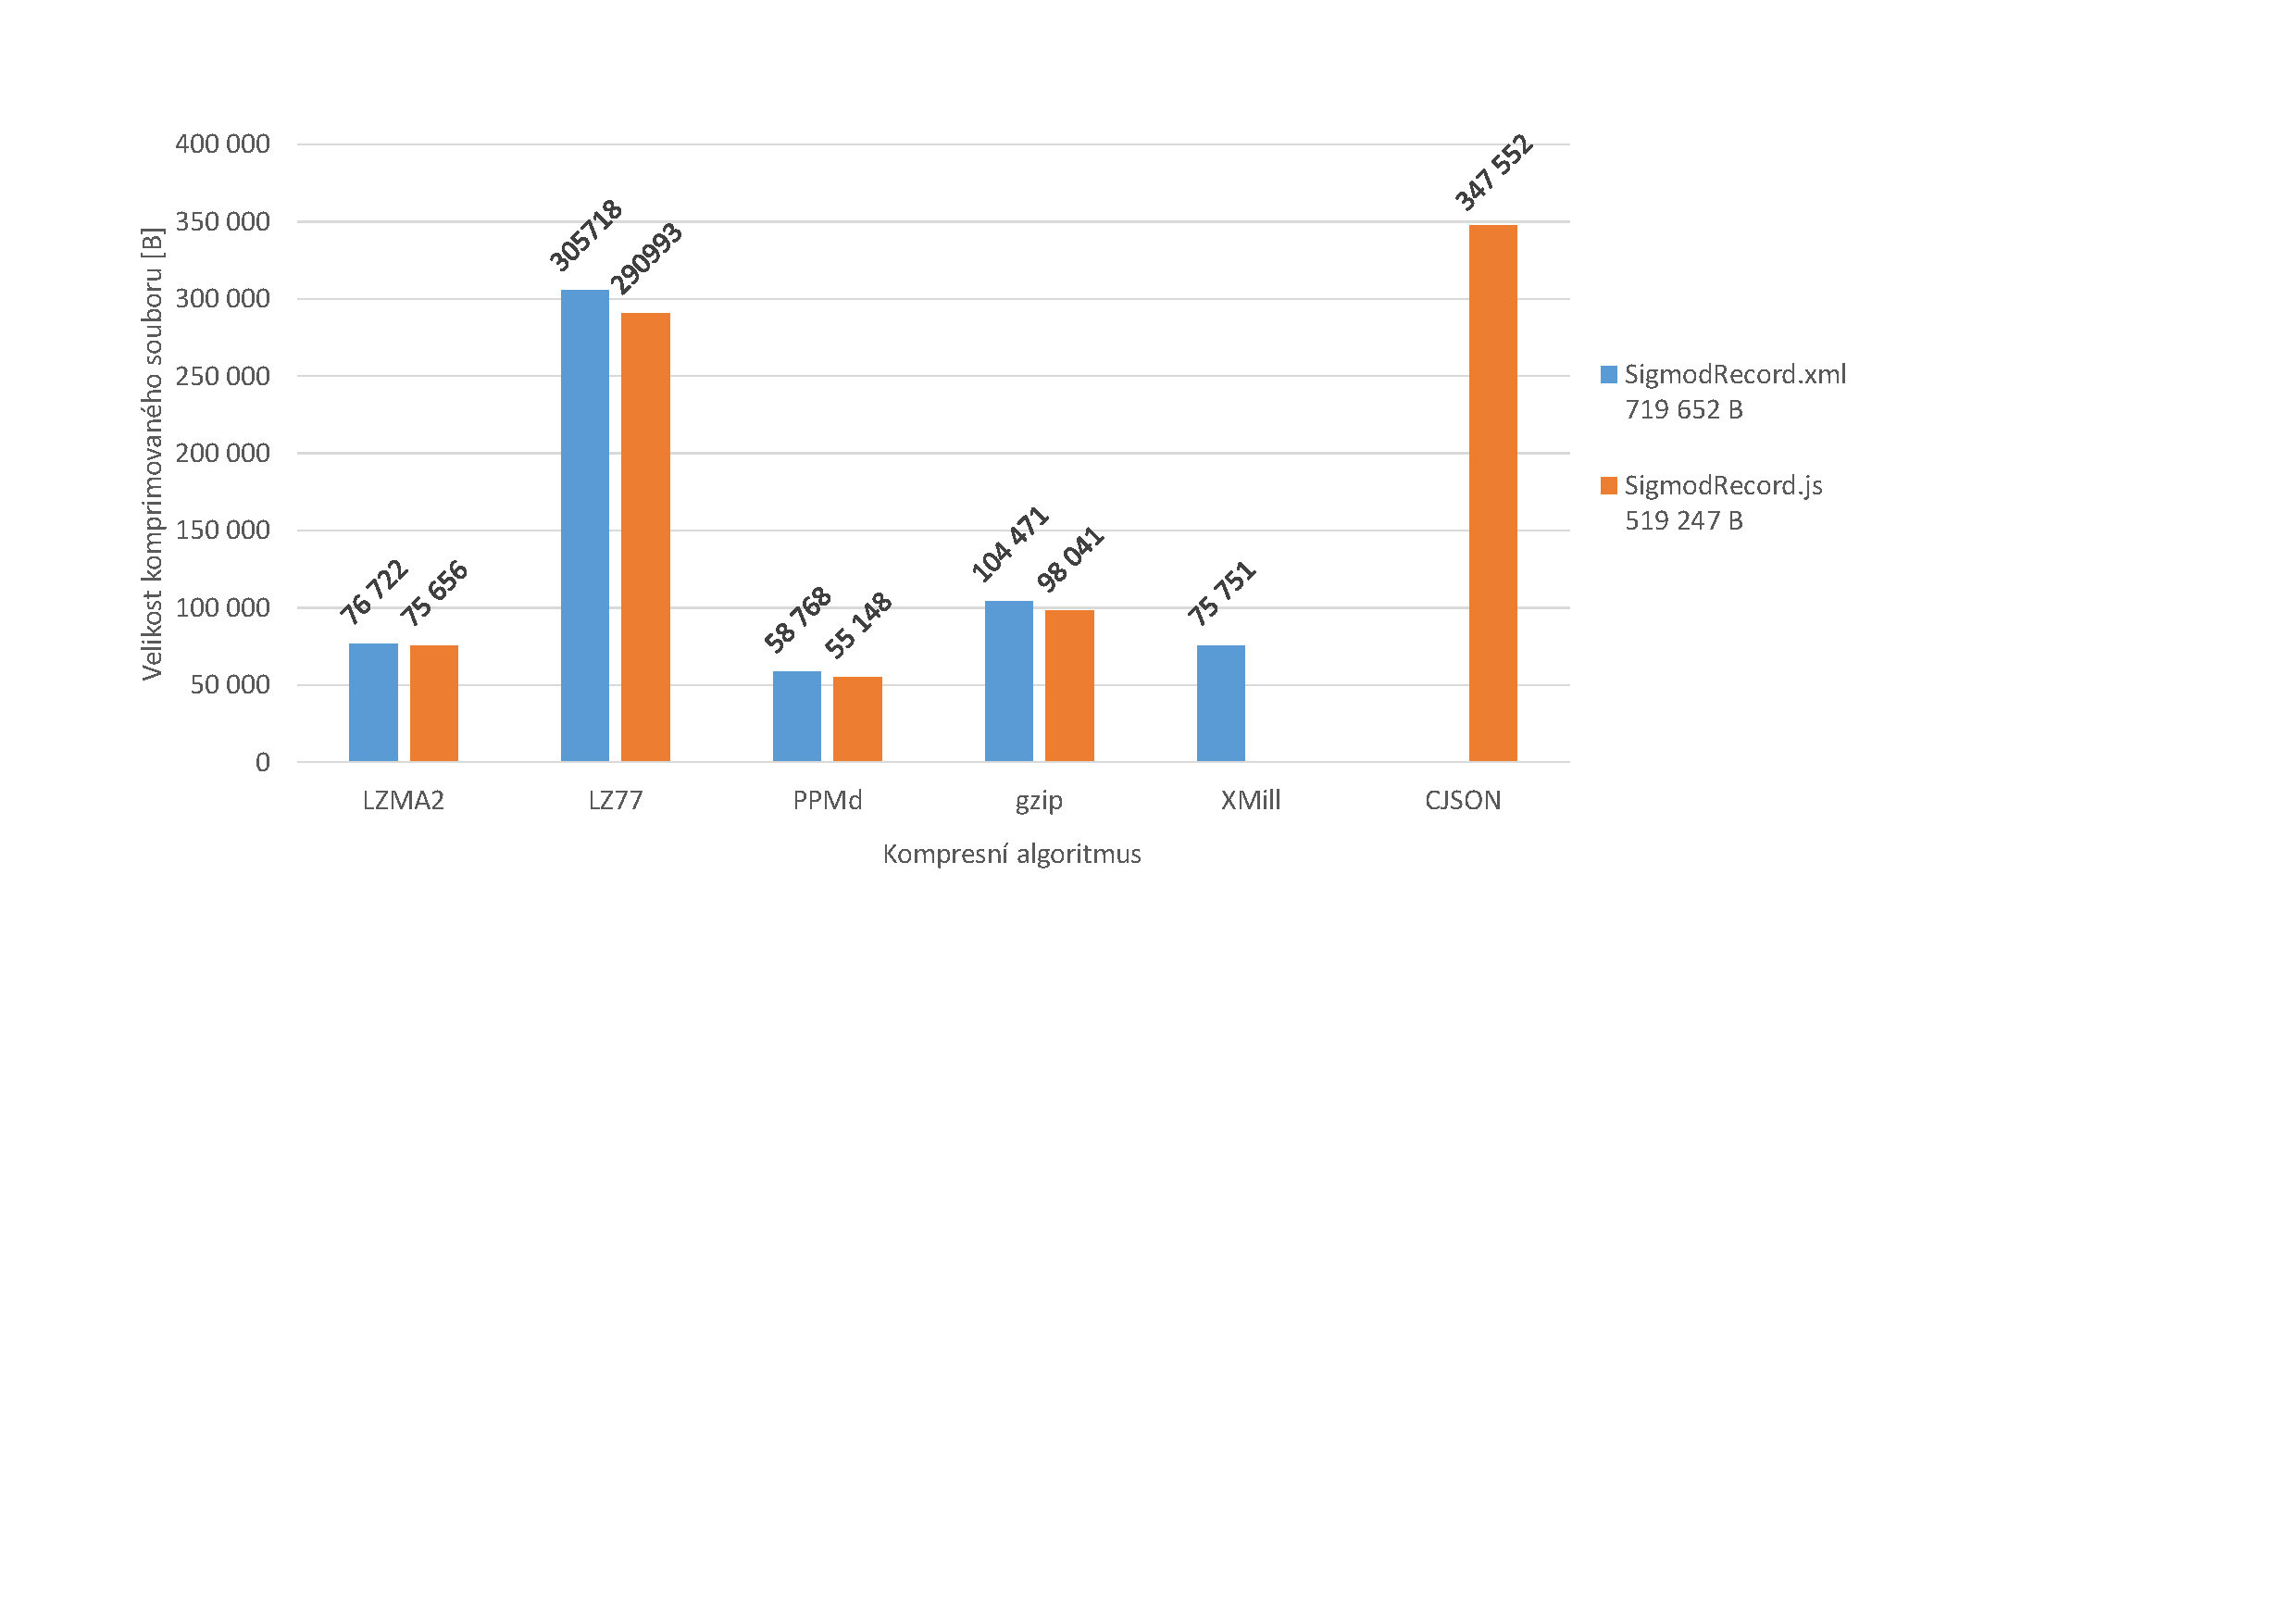
\includegraphics[trim=70 380 200 60, clip, angle=0, width=140mm]{SigmodRecord}
\caption{Velikost komprimovaných souborů SigmodRecord.xml a SigmodRecord.js}
\label{SigmodRecord}
\end{figure}

\clearpage
\subsection{Kompresní poměr}
V tabulce \ref{tabulkaKompresniPomer} jsou uvedeny nejvyšší získané kompresní poměry pro soubor a kompresní metodu. Pro soubor Employees.xml dosáhly všechny použité metody vysokého kompresního poměru, z nichž nejvyššího 46,33 dosáhla metoda PPMd, tato hodnota odpovídá téměř 98\% úspoře místa. Nižší kompresní poměr souborů JSON než jejich XML alternativ je dán nižší redundancí formátu JSON.

\begin{table}[!h]
\catcode`\-=12
\centering
\begin{tabular}{|l|r|r|r|r|r|r|r|}
\hline
 \multirow{2}{*}{Soubor} & \multicolumn{7}{|c|}{Kompresní poměr algoritmu}\\
 \cline{2-8}
 & LZMA2 & LZ77 & PPMd & gzip & XMill & JSONH & CJSON\\
 \hline
 base64img.xml & 3,28 & 1,28 & 3,30 & 3,30 & 3,28 & & \\
 base64img.js & 3,24 & 1,50 & 3,26 & 3,26 & & 1,04 & 1,01\\
 \hline
 dblp.xml & 6,63 & 1,61 & 7,98 & 6,07 & 5,97 & & \\
 dblp.js & 5,53 & 1,45 & 6,49 & 5,30 & & & 1,23\\
 \hline
 Employees.xml & 26,80 & 4,76 & 46,33 & 21,06 & 30,35 & & \\
 Employees.js & 17,35 & 3,23 & 28,62 & 14,35 & & 2,77 & 2,40\\
 \hline
 nasa.xml & 10,95 & 1,33 & 13,20 & 6,94 & 8,17 & & \\
 nasa.js & 8,30 & 0,77 & 9,76 & 5,44 & & & 1,17\\
 \hline
 SigmodRecord.xml & 9,38 & 2,35 & 12,26 & 6,89 & 9,50 & & \\
 SigmodRecord.js & 6,87 & 1,78 & 9,42 & 5,30 & & & 1,49\\
\hline
\end{tabular}
\caption{Kompresní poměr vybraných algoritmů na testovacích souborech}
\label{tabulkaKompresniPomer}
\end{table}

\subsection{Hodnocení algoritmu LZ77}
Testování vlastní implementace LZ77 nepřineslo příliš dobré výsledky. V měřených charakteristikách končí daleko za ostatními obecnými algoritmy. Pro soubor nasa.js dosáhl dokonce kompresního poměru menšího než 1, tedy došlo k nárůstu objemu dat. Přitom při kompresi tohoto souboru dosáhly ostatní algoritmy nadprůměrného výsledku. Další jeho nepříjemnou vlastností je dlouho trvající proces komprese a ještě déle trvající proces dekomprese.

Za nejpravděpodobnější příčinu považuji malou velikost slovníku a příliš častý zápis malého množství dat do souboru. Ke zvolenému nastavení jsem ale dospěl ve snaze vyvarovat se nadměrné spotřeby paměti, což se podařilo. Vzhledem k tomu, že smyslem práce nebylo vytvořit dokonalý kompresní algoritmus, ale spíše si prakticky vyzkoušet danou problematiku, považuji dosažené výsledky za uspokojivé.

\subsection{Porovnání výsledků}
Srovnáváme-li soubory po dvojicích, tedy vždy XML a JSON obsahující stejná data, lze pozorovat jisté trendy. Prvním z nich je, že soubor s JSON je vždy menší než soubor s~XML. To je dáno tím, jak již bylo napsáno v kapitole \ref{kapitolaXmlAJson}, že JSON vznikl jako odlehčená alternativa ke XML a tedy neobsahuje tolik redundance. Dalším zajímavým pozorováním je, že ač se testovací soubory obsahující stejná data v XML a JSON liší významně velikostí, tak zkomprimované soubory mají přibližně stejnou velikost.

Účinnost kompresních algoritmů pro obecná data je velmi vysoká pro oba zkoumané formáty. Metoda PPMd dokonce algoritmy využívající znalosti struktury dat značně pře\-ko\-ná\-vá. Pokud bychom se zajímali pouze o velikost komprimovaných souborů, potažmo kompresní poměr, nelze ke kompresi doporučit specializované algoritmy popsané v kapitolách \ref{kapitolaXmlAlgoritmy} a \ref{kapitolaJsonAlgoritmy}. Pokud ale potřebujeme s komprimovanými daty pracovat (např. dotazování do zkomprimovaných dat, viz \ref{xgrind}), nezbývá nám, než tyto specializované algoritmy použít. Je to ale vykoupeno nižším kompresním poměrem.

Rozhodnutí, zda je výhodnější komprimovat data ve formátu XML nebo JSON, není tak jednoznačné, jak jsem na začátku práce předpokládal. V porovnání původních souborů jsou jasně menší soubory JSON, zatímco komprimované testovací soubory se velikostí liší v řádu jednotek procent. Výhodnost využití znalosti struktury dat se nepodařilo prokázat. Na základě uvedených poznatků považuji za úspornější, tzn. vhodnější k archivaci a přenosu dat, formát JSON.